\documentclass{acmsiggraph}
\usepackage{mathptmx}
\usepackage{graphicx}
\usepackage{epsfig}
\usepackage{amsmath,amscd,amssymb}
\usepackage{hyperref}

\newtheorem{theorem}{Theorem}[section]
\newtheorem{proposition}[theorem]{Proposition}
\newtheorem{definition}[theorem]{Definition}
\newtheorem{lemma}[theorem]{Lemma}
\newtheorem{corollary}[theorem]{Corollary}
\newtheorem{remark}[theorem]{Remark}

\usepackage{parskip}

\onlineid{papers\_0142}

\acmformat{cameraready}

\title{CS 555 Term Project Proposal: Visualizing the Loss Landscape of Neural Nets}

\author{Charles Ison\thanks{\small\texttt{e-mail: \{isonc|morgamat\}@eecs.oregonstate.edu}}\\ Oregon State University
\and Matthew Morgan$^{\ast}$ \\
Oregon State University}

\keywords{loss landscape, scalar field topology, neural networks, gradient descent}

\begin{document}

\teaser{
	%\centerline{\epsfig{file=images/teaser.eps,angle=0,width=\textwidth}}
	$\begin{array}{@{\hspace{-0.00in}}c@{\hspace{0.05in}}c@{\hspace{0.05in}}c@{\hspace{0.05in}}c}
			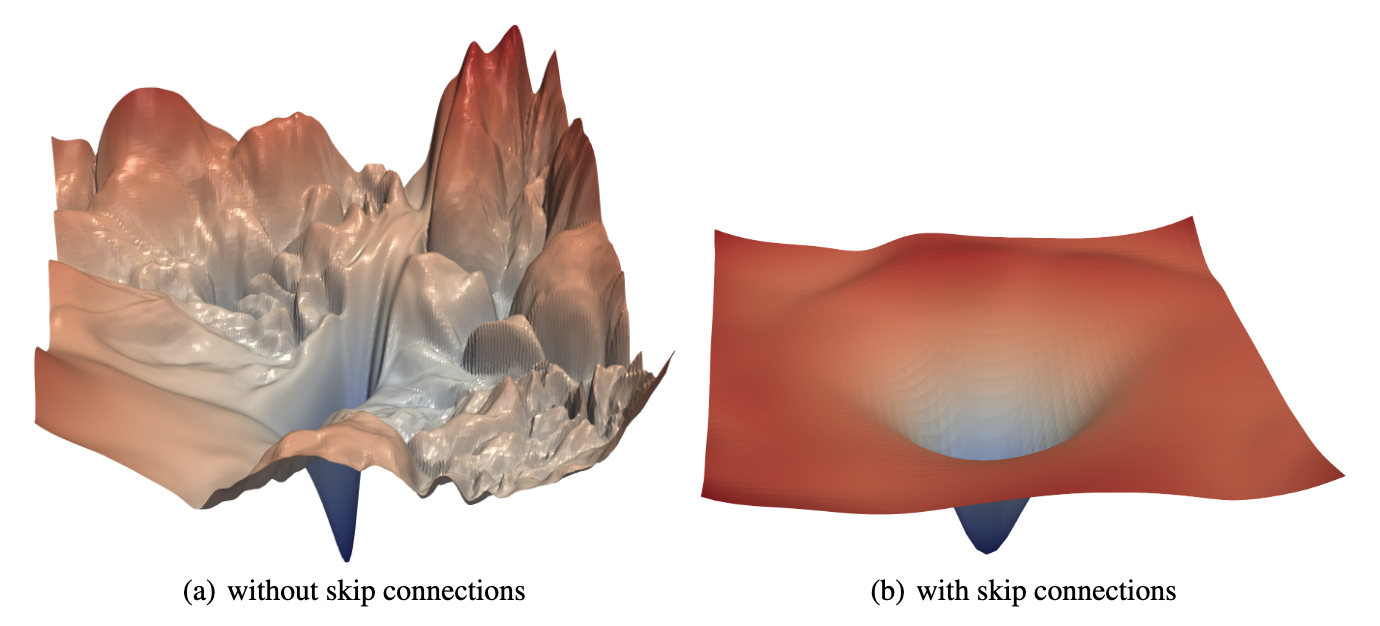
\includegraphics[width=5.50in]{images/scalar-field-teaser.png}
			\\
		\end{array}$
	\caption{Two visualizations from the proposed paper: (a) the loss function of a neural network architecture without skip connections, and (b) with skip connections.
		We propose to implement these visualizations as the first step of our term project, then proceeding with creating other visualizations and enhancing them. } \label{fig:teaser} }

\maketitle
\keywordlist

\section{Paper Proposal}
\label{sec:intro}

For our term project, we propose to use the paper "Visualizing the Loss Landscape of Neural Nets" (\url{https://arxiv.org/pdf/1712.09913.pdf}) for Option 2 (implementing a published research paper). In this paper, the authors create scalar field visualizations of various neural network architectures that they call “Loss Landscapes.” In these visualizations, the loss function’s results serve as the scalar value and a two dimensional reduction of the model’s weights serves the directional elements of the field. The specific loss functions used in the original paper are cross entropy (\url{https://pytorch.org/docs/stable/generated/torch.nn.CrossEntropyLoss.html}) and mean squared error (\url{https://pytorch.org/docs/stable/generated/torch.nn.MSELoss.html}).
The dimensionality reduction is done using two different approaches: principal component analysis and random vector selection. For the later approach, two random vectors within the input space are created by sampling a random Gaussian distribution. These vectors are used as the two dimensions of the scalar field input. The resulting loss landscapes generated can then provide insights into how certain architectural decisions can improve or worsen a network's trainability.

\section{Data Sets}
\label{sec:intro}

Just like the original authors, we will have to generate our own datasets by creating test models of multiple popular neural network architectures and recording their performance across a range of weights. The original authors tested ResNet and VGG architectures with various permutations, which we can recreate and also potentially extend to newer architectures such as a Vision Transformer (\url{https://arxiv.org/pdf/2010.11929v2.pdf}). To create our loss dataset, we will also use the CIFAR-10 dataset (\url{https://www.cs.toronto.edu/~kriz/cifar.html}) as input into our testing models like the original paper. The models will be created in Python using PyTorch and then our results exported to PLY files which we will use to generate corresponding visualizations in OpenGL.


\section{Visualization Evaluation}
\label{sec:intro}
To validate the correctness of our models we will use four criteria:
\begin{enumerate}
	%\itemsep 0pt
	%\parskip -1pt
	\item We will confirm that our model's results align with the original papers, which includes both quantitatively confirming the performance is as expected and visually confirming our loss landscapes align with those presented in the paper.
	\item Then, we will extract all critical points from our field, classify them using a Hessian, and confirm they match the expected values based on the scalar field visualization.
	\item Next, the original authors visualized their model’s convergence to a local minimum during gradient descent. We will do the same using polylines in OpenGL and then confirm the convergence’s path both matches our model’s results and follows the expected path of least resistance along our scalar field.
	\item Finally, we will judge our visualization’s overall usefulness by the ability to draw meaningful insights about neural network’s architectures from the visualization. For example, the original authors were able to gain an intuition about the impact of increasing network depth and its impact on convexity. Our visualizations should be of a high enough quality to convey the same information.
\end{enumerate}


\begin{figure}[t]
	\begin{center}
		$\begin{array}{@{\hspace{-0.00in}}c@{\hspace{0.05in}}c}
				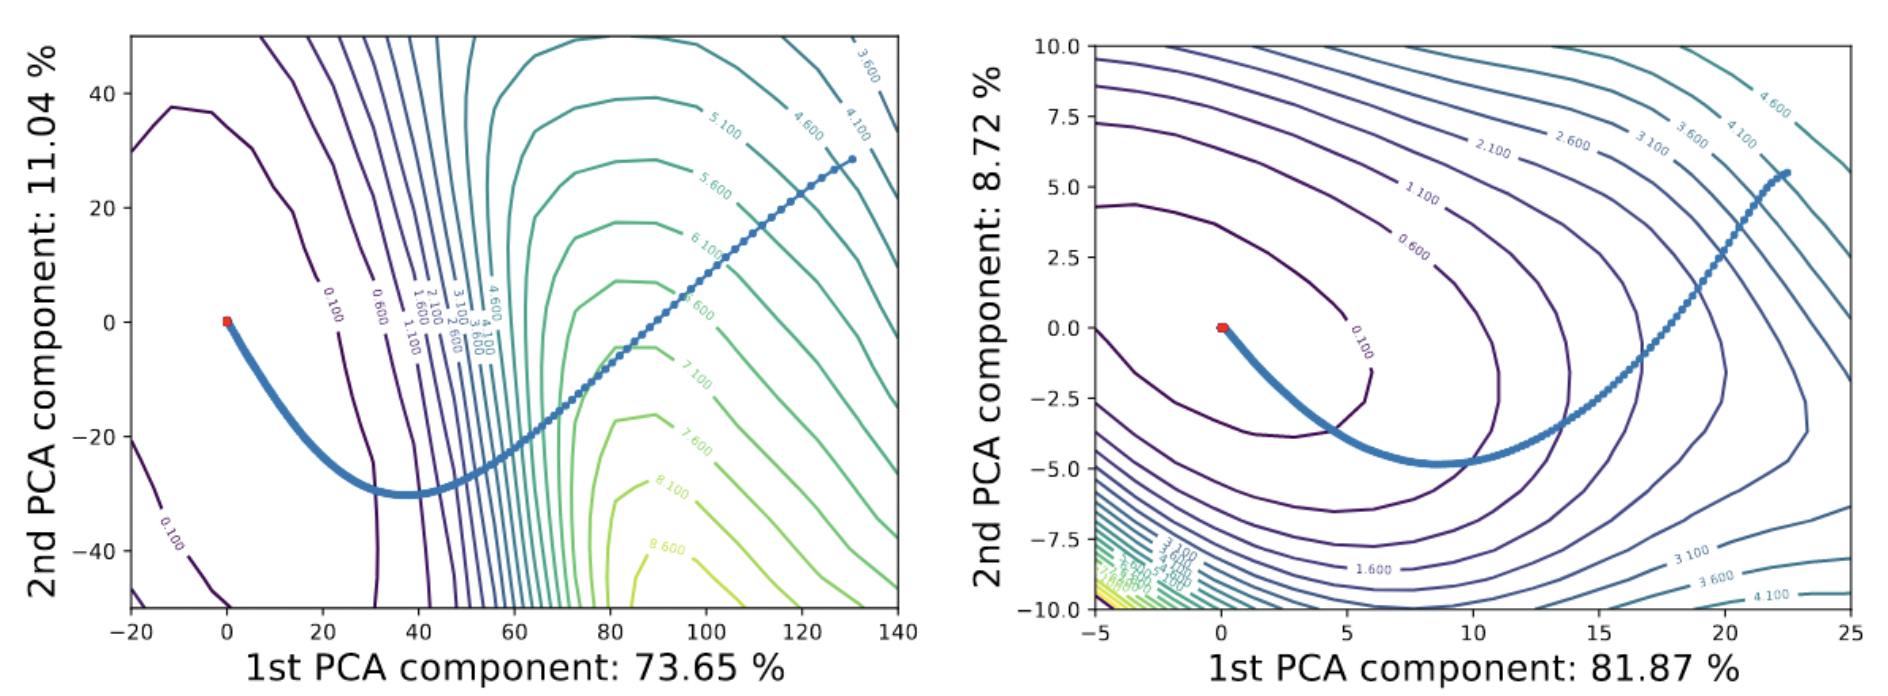
\includegraphics[height=1.07in]{images/traj-plot-SGD.png}
				\\
			\end{array}$
	\end{center}
	\caption{ Plots from the original authors visualizing the model's convergence to a local minimum during gradient descent. } \label{fig:descent_trajectory}
\end{figure}



\section{Related Work}
\label{sec:previous_work}

There have been numerous studies on the ability to optimize neural loss functions in order to improve training time and model performance. Less work has been conducted on visualizing the losses though to gain intuition about how certain architectural decisions impact the loss field's convexity. However, one paper by ~\cite{hochreiter1997flat} defined “flatness” as the size of the connected region around the minimum where the training loss remains low which is visualized by this work. Since the paper was released in 2018, numerous other works have cited it. However, many of the citations are not from works attempting to advance the visualizations, but rather to learn from the visualizations and develop more generalizable and accurate models. The visualizations have come in handy for researchers studying reinforcement learning models such as \cite{actor2020} and \cite{plaat2022deep}.

There are some recent works which produce new visualizations of loss functions. One such by ~\cite{pmlr-v137-huang20a}, "Understanding Generalization Through Visualizations", use
visualization methods to give intuitions about why certain architectures generalize better than others. They first visualize loss as a scalar field with height and color representing the output. But they also use a colored dot plot and a "Swissroll decision boundary" to show the difference in models that perform well versus models that perform poorly at generalizing.

An interesting extension of this work by ~\cite{linse2022walk} visualizes large neural networks in virtual reality. The approach allows for high interactivity, but requires a virtual reality headset and powerful computer to render.

\bibliographystyle{acmsiggraph}
\nocite{*}
\bibliography{nn_loss}
\end{document}
